\chapter{Routing Analysis and Ablation}\label{ch:routing}
% LENGTH: 7-9 pages. This is where the project's real contribution lives.
% SOURCES: results/diagnostics/{summary,routing}.json, interventions.csv,
% results/phase4/jobs.json, fcsg-report-assets/live_*.
% RULES:
%  - Correlation is not specialisation. 36 exploratory correlations, 10 source
%    images, no multiple-comparison correction. Say that next to the numbers.
%  - Inference interventions are NOT ablations. Keep them in separate sections.

\section{Spatial Routing Statistics}\label{sec:routing-stats}
% routing_summary.pdf (80 samples = 10 images x 8 seeds).
% High band picks the 3x3 expert almost always (0.999845) yet 7x7 and 5x5 still
% carry ~0.256 and ~0.223 mean weight there.
\begin{figure}[htbp]
	\centering
	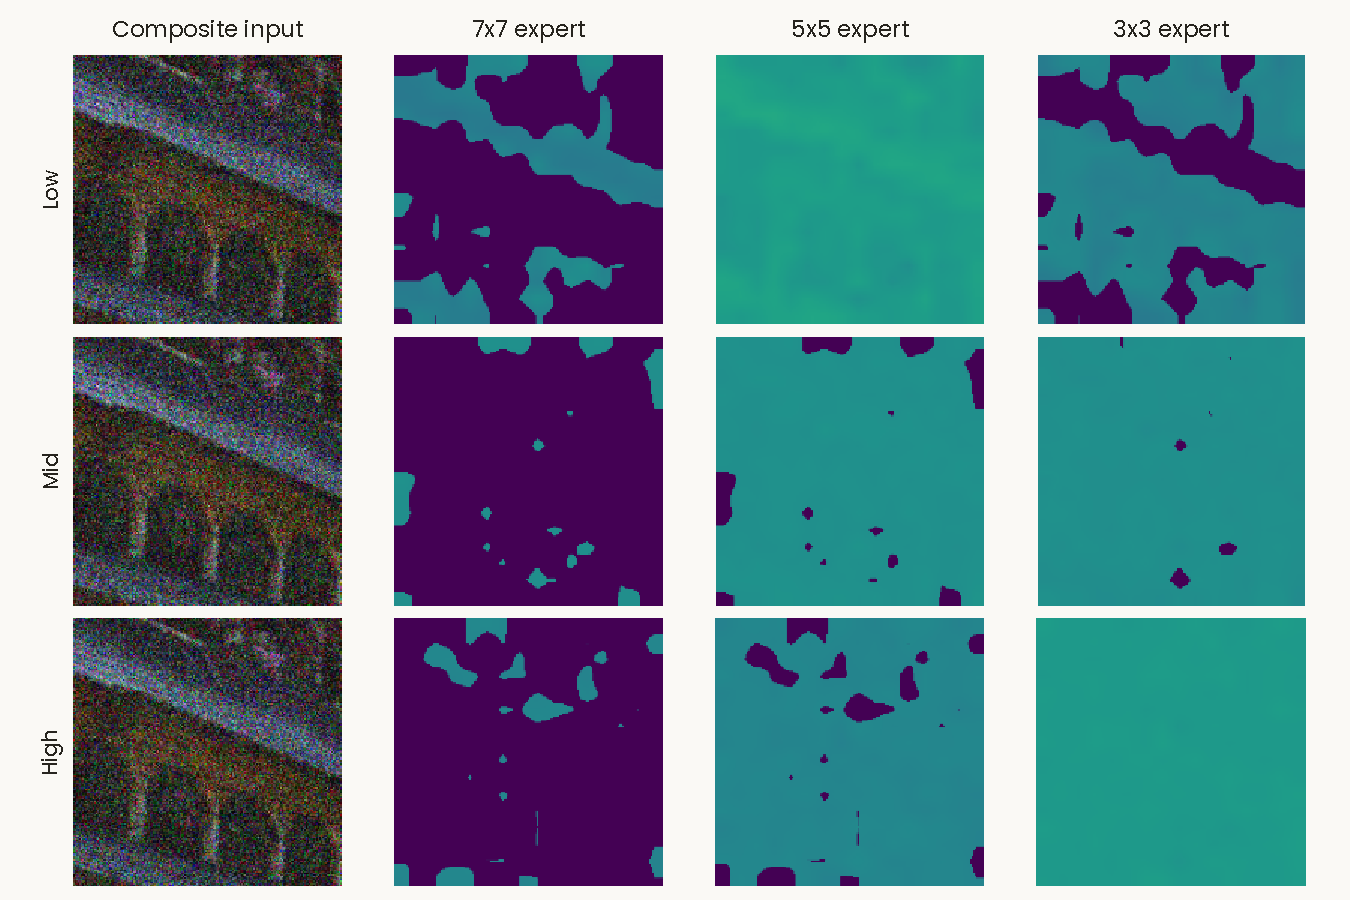
\includegraphics[width=\linewidth]{routing_0834.pdf}
	\caption{Per-band expert weights for DIV2K image 0834. Rows: low, mid, high band.}
	\label{fig:routing-map}
\end{figure}
\todo{write}

\section{Routing Versus Degradation Parameters}\label{sec:routing-corr}
% Within-image-centred Pearson r: high-band 3x3 vs noise sigma +0.809;
% low-band 5x5 +0.798; low-band 7x7 -0.728. Figure correlations_interventions.pdf.
\todo{write, with the caveats above}

\section{Inference-Time Interventions}\label{sec:interventions}
\begin{table}[htbp]
	\centering
	\caption{PSNR change when the trained gate is overridden at inference (10 images).}
	\label{tab:interventions}
	\evidence{results/diagnostics/interventions.csv}
	\begin{tabular}{@{}lrr@{}}
		\toprule
		Intervention & Mean $\Delta$PSNR & Min / Max \\
		\midrule
		Equal weights on selected pair    & $-0.040$\dB & $-0.137$ / $+0.028$ \\
		Uniform weights over all experts  & $-0.372$\dB & $-0.986$ / $+0.163$ \\
		\bottomrule
	\end{tabular}
\end{table}
% Reading: the model depends on WHICH pair it picks far more than on the
% exact mixing weights. That is a useful, specific finding.
\todo{write}

\section{Trained Routing Ablation}\label{sec:ablation}
% fcsg_reference vs fcsg_uniform, seed 1234, 100k steps, matched init.
% STATUS CHECK BEFORE WRITING: results/phase4/jobs.json was last updated
% 2026-10-01 with both runs RUNNING. Pull the finished Kaggle outputs, run the
% 100-image eval, and fill this table. If the runs did not finish, report the
% interim crop numbers as interim and move the conclusion to future work.
\begin{table}[htbp]
	\centering
	\caption{Learned top-2 routing against fixed uniform mixing, matched training.}
	\label{tab:ablation}
	\begin{tabular}{@{}lrrrr@{}}
		\toprule
		Variant & PSNR & SSIM & LPIPS & Trainable params \\
		\midrule
		Reference (learned top-2) & \todo{} & \todo{} & \todo{} & 97,088 \\
		Uniform ($w=1/3$)         & \todo{} & \todo{} & \todo{} & 96,407 \\
		\bottomrule
	\end{tabular}
\end{table}
% Note the ablation removes routing AND entropy regularisation together.
\todo{write once numbers exist}

\section{Discussion}\label{sec:discussion}
% Pull Ch 5 and Ch 6 together: what did routing buy, what did it cost?
% The interventions say the gate matters to THIS checkpoint; only the
% ablation says whether learning a gate beats not having one.
\todo{write}
